\section{Introducción}
Una vez elegido el tipo de asistente virtual inteligente en el capítulo previo, en el presente capítulo se procede al análisis tanto de requisitos que debe cumplir el sistema, como de las funcionalidades que debe tener la página de administración, pasando por las operaciones que debe de ser capaz de realizar el dispositivo.

\section{Requisitos}

Para poder identificar qué es lo que se debe implementar, se debe realizar primero una identificación de las necesidades técnicas del proyecto a desarrollar, con el fin de identificar cuales son las implementaciones que se deben desarrollar.

\subsection{Requisitos funcionales}

Los requisitos funcionales son un conjunto de funciones que debe poder servir el proyecto. Están basados en especificar qué es lo que el sistema debe ser capaz de hacer o permitir, y son los siguientes:

    \begin{enumerate}
    \item Los dispositivos deben ser capaces de identificarse ante el sistema.

    \item El sistema debe permitir obtener un nuevo token de acceso mediante un token de refresco.

    \item El sistema debe ser capaz de registrar nuevos dispositivos.

    \item El sistema debe devolver un par de tokens de autenticación a los dispositivos que se identifiquen.

    \item El dispositivo debe informar al sistema sobre su estado cada un cierto tiempo, que pueda ser configurable, siendo guardado en un fichero de configuración.

    \item El sistema debe poder actualizar remótamente el archivo de configuración tanto de dispositivos particulares, como de dispositivos de una misma localidad, como de todos los dispositivos en conjunto.

    \item El sistema debe poder asignar tareas a un dispositivo, a una localidad, o a todos los dispositivos.

    \item El sistema debe ser capaz de mandar tareas pendientes a realizar a un dispositivo, como puede ser actualizar su archivo de configuración, apagar el dispositivo, o reiniciarlo, cuando el dispositivo informe de que esté conectado.

    \item El dispositivo debe realizar las tareas por fecha de creación.

    \item El dispositivo debe informar al sistema cada vez que proceda a realizar una tarea.

    \item El sistema debe poder marcar tareas de un dispositivo específico como ya realizadas, guardando la fecha de realización.

    \item El sistema debe ser capaz de recibir la información básica sobre una conversación entre el asistente y el usuario, para monitorizar su uso.

    \item El dispositivo debe avisar al sistema sobre conversaciones que haya tenido con el usuario, mandando la información básica que confronte con los hechos.

    \item El sistema tiene que ser capaz devolver información básica sobre una localidad, como el número de teléfono, direcciones de correo, y noticias en función de la ubicación del dispositivo que llame al servicio.
    
    \item Un administrador debe poder iniciar sesión, identificandose a continuación mediante tokens.
    
    \item Un administrador debe ser capaz de ver todos los tipos de tareas disponibles.
    
    \item Un administrador debe poder crear nuevos tipos de tareas.
    
    \item El dispositivo debe tener un protocolo de adicción de nuevas tareas, de manera que al añadir una nueva tarea no haya posibilidad de afectar al resto ya implementadas.
    
    \item Un administrador debe poder asignar tareas a dispositivos especificos, a dispositivos de una localidad específica, o a todos los dispositivos en general.
    
    \item Un administrador debe poder ver las tareas pendientes de un dispositivo específico.
    
    \item Un administrador debe poder cambiar la configuración a dispositivos especificos, a dispositivos de una localidad específica, o a todos los dispositivos en general.
    
    \item Un administrador debe poder obtener una lista de todos los dispositivos, incluyendo estos sus últimos estados, últimas tareas realizadas, tareas pendientes, e información sobre el usuario asignado.
    
    \item Un administrador debe poder ver la actividad ocurrida en un intervalo específico de tiempo de un dispositivo sin asignar.
    
    \item Un administrador no debe poder ver actividad de un usuario que ya no tenga un dispositivo asociado.
    
    \item Un administrador debe poder ver la actividad de un dispositivo asignado ocurrida en un intervalo específico de tiempo cuya fecha mínima sea la fecha en que se estableció la asignación.
    
    \item Un administrador debe poder añadir nuevas localidades al sistema, incluyendo su nombre, coordenadas, y código postal.
    
    \item Un administrador debe poder obtener la lista de localidades almacenadas en el sistema, teniendo cada localidad información sobre los dispositivos asignados a clientes.
    
    \item Un administrador debe poder añadir nuevos clientes, que representarán a los poseedores del dispositivo. 
    
    \item Un administrador debe poder obtener la lista de clientes.
    
    \item Un administrador debe poder asignar un dispositivo a un cliente específico.
    
    \item Un administrador debe poder desasignar un cliente de un dispositivo.
    
    \item Un administrador debe ser capaz de poder ver cuales son las acciones que más se le han solicitado a un dispositivo, y las estadísticas de a qué horas ha sido más veces consultado.

\end{enumerate}




\subsection{Requisitos no funcionales}

Los requisitos no funcionales, al contrario de los descritos en el apartado anterior, se basan en la descripción de cómo esta implementado el sistema y sobre cómo debe interacturar.

    \begin{enumerate}

    \item La base de datos debe ser una base de datos de tipo relacional, preferiblemente usando PostgreSQL.
    
    \item El backend debe estar implementado con un lenguaje que pueda ser ejecutado bajo la JVM.
    
    \item Las contraseñas que se almacenen en el sistema deben estar encriptadas mediante una encriptación de tipo SALT.
    
    \item El administrador debe poder ver la ubicación de los dipositivos a través de un mapa implementado con Leaflet y OpenMaps.
    
    \item De un cliente se debe almacenar su código postal, nombre, apellidos y número de documento nacional de identidad.
    
    \item En la web administrativa, un dispositivo SIN cliente asignado debe aparecer en el mapa ubicado en la costa atlántica, con el icono en color amarillo.
    
    \item En la web administrativa, un dispositivo CON cliente asignado debe aparecer en el mapa ubicado en la posición de su localidad, con el icono en color verde.
    
    \item En la web administrativa, todos los dispositivos de una localidad deben aparecer en el mapa agrupados, ocultando sus iconos y mostrando el número de ellos que hay en ese grupo.
    
    \item En la web administrativa, al hacer click en un grupo de dispositivos del mapa, se debe mostrar el icono de cada dispositivo en color verde.
    
    \item En la web administrativa, al hacer click en un icono del mapa, debe salir información sobre el cliente asignado, y un enlace a para ver sus estadísticas.
    
    \item El periodo de filtración de las estadísticas en la web administrativa debe ser de un día específico, o de un mes específico, o de un año específico.
    
    \item Las estadisiticas de acciones de un dispositivo deben ser mostradas en la web administrativa en un diagrama de tipo Doughnut, y las horas de uso en un diagrama de barras.
    
    \item La web administrativa debe tener un panel donde se vean los dispositivos mediante tarjetas, que cambien de color en función de tiempo que lleve el dispositivo sin ser usado.
    
    \item La web administrativa debe permitir filtrar las tarjetas en función de si los dispositivos están asignados, de su última fecha de uso, y de la última fecha de tarea realizada, mostrando cuánto tiempo hace de su último uso.
    
    \item La web administrativa debe permitir asignar tareas a los dispositivos de una manera rápida dando click a una tarjeta, al igual que dar acceso rápido al apartado de estadísticas y configuraciones, y mostrar información del usuario asignado.
    
\end{enumerate}

\section{Riesgos}

        \subsection{Introducción}
        A continuación, se analizarán los posibles riesgos, siendo estos los posibles problemas futuros que puedan tener un efecto positivo o negativo en los objetivos del proyecto, incluyendo cada uno de ellos un conjunto de causa-efectos.
        
        Para tratar mejor un riesgo, hay que tener en cuenta dos aspectos: cuál es la probabilidad de que ocurra, y cuál es el impacto que tendría en el proyecto en caso de que ocurriese.
        Una vez estimadas estas dos variables, se puede asignar una posición de ese riesgo dentro de la matriz de la figura \ref{fig:riskmatrix}.
        
        Una vez asignada su posición, se deberá priorizar todo riesgo que ocupe una posición superior a la línea de tolerancia, por ejemplo, los riesgos R1 y R6 representados en la figura \ref{fig:riskmatrix}.
        
        \begin{figure}[H]
            \centering
            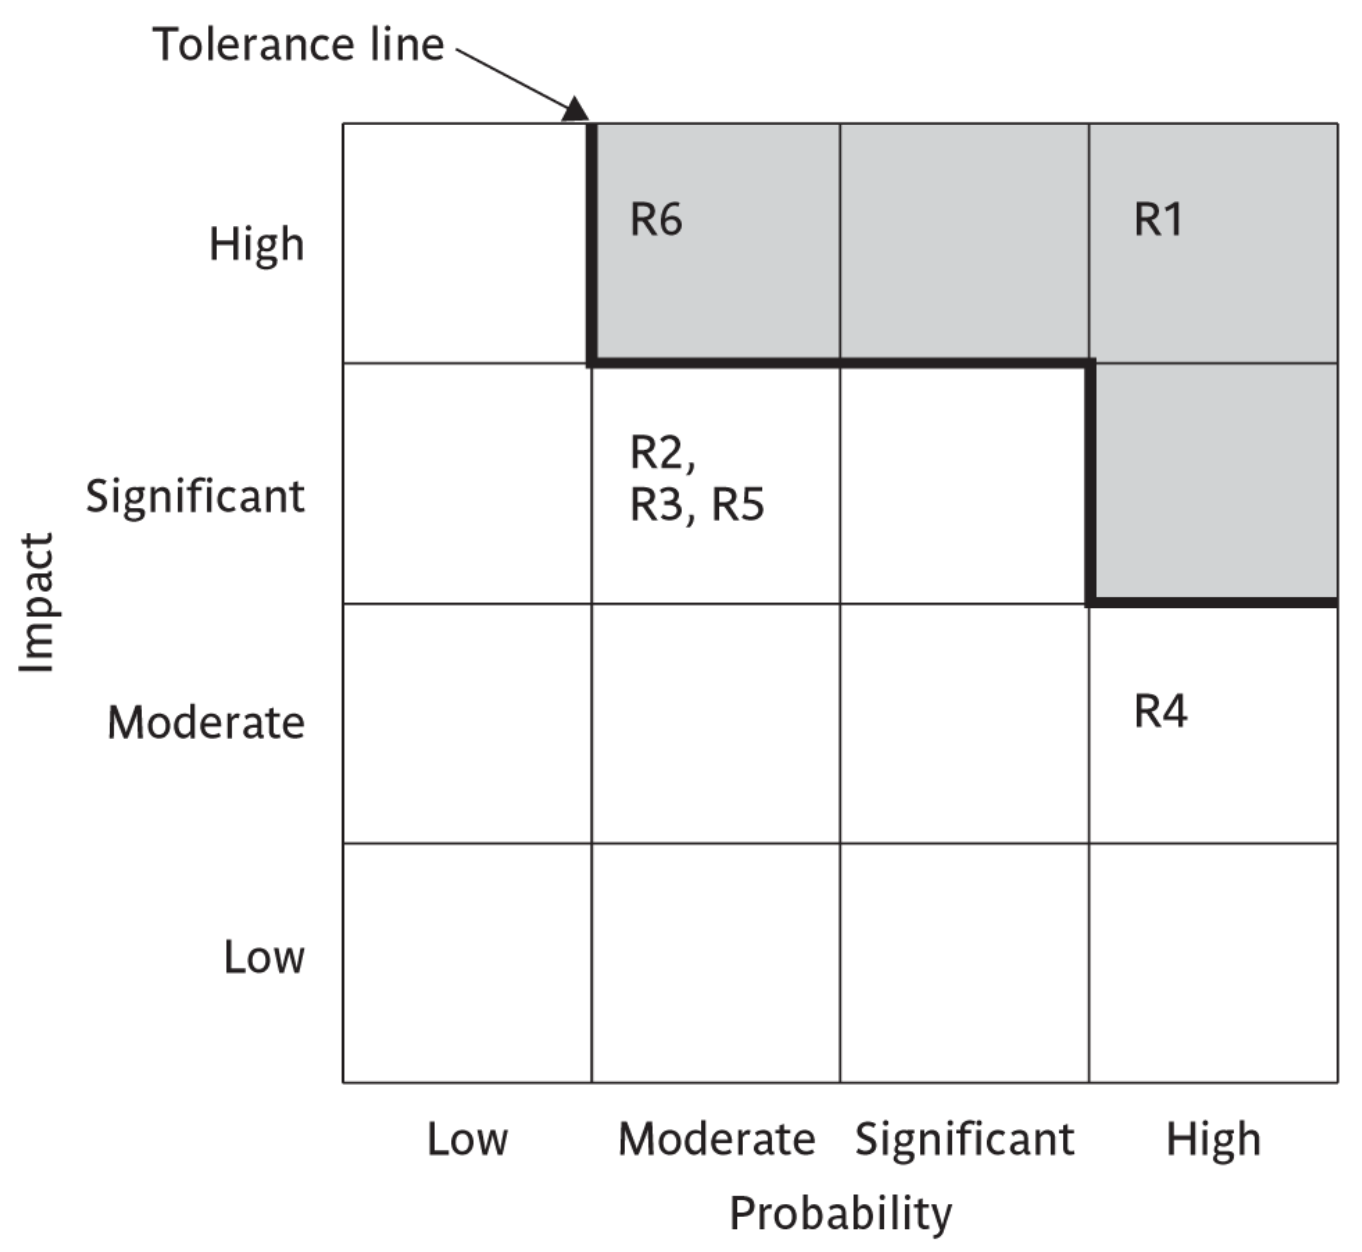
\includegraphics[width=6cm]{./img/spm/riskmatrix.png}
            \caption{Matriz de priorización de riesgos}
            \label{fig:riskmatrix}
        \end{figure}

\newpage
    \subsection{Riesgos identificados}
        A continuación se clasifican los riesgos que pueden tener un impacto sobre el proyecto:
        %t1
        \begin{table}[H]
        \centering
        \begin{tabular}{|l|c}
        \hline
        \textbf{Riesgo}               & \multicolumn{1}{r|}{R-01}                                             \\ \hline
        \textbf{Descripción}          & \multicolumn{1}{X|}{El desarrollador puede enfermar debido a las  condiciones externas.}
        \\ \hline
        \textbf{Impacto}              & \multicolumn{1}{r|}{SIGNIFICANTE}                                             \\ \hline
        \textbf{Probabilidad}         & \multicolumn{1}{r|}{MODERADA}                                         \\ \hline
        \textbf{Plan de mitigación}   & \multicolumn{1}{X|}{Evitar acciones que atenten contra la salud. }
        \\ \hline
        \textbf{Plan de contingencia} & \multicolumn{1}{X|}{Trabajo desde casa.}
        \\ \hline
        \end{tabular}
        \caption{Riesgo 01 - Enfermedad}
        \label{table:riskill}
        \end{table}
        % t2
        \begin{table}[H]
        \centering
        \begin{tabular}{|l|c}
        \hline
        \textbf{Riesgo}               & \multicolumn{1}{r|}{R-02}                                             \\ \hline
        \textbf{Descripción}          & \multicolumn{1}{X|}{Mala planificación del proyecto.}
        \\ \hline
        \textbf{Impacto}              & \multicolumn{1}{r|}{SIGNIFICANTE}                                             \\ \hline
        \textbf{Probabilidad}         & \multicolumn{1}{r|}{MODERADA}                                         \\ \hline
        \textbf{Plan de mitigación}   & \multicolumn{1}{X|}{Reuniones cada dos semanas de seguimiento }
        \\ \hline
        \textbf{Plan de contingencia} & \multicolumn{1}{X|}{Aumentar el tiempo de trabajo hasta alcanzar lo planeado.}
        \\ \hline
        \end{tabular}
        \caption{Riesgo 02 - Planificación incorrecta}
        \label{table:malaplanif}
        \end{table}
        % t3
        \begin{table}[H]
        \centering
        \begin{tabular}{|l|c}
        \hline
        \textbf{Riesgo}               & \multicolumn{1}{r|}{R-03}                                             \\ \hline
        \textbf{Descripción}          & \multicolumn{1}{X|}{Pérdida del trabajo elaborado.}
        \\ \hline
        \textbf{Impacto}              & \multicolumn{1}{r|}{ALTO}                                             \\ \hline
        \textbf{Probabilidad}         & \multicolumn{1}{r|}{BAJA}                                         \\ \hline
        \textbf{Plan de mitigación}   & \multicolumn{1}{X|}{Utilización de varios servicios de control de versiones. }
        \\ \hline
        \textbf{Plan de contingencia} & \multicolumn{1}{X|}{Recuperar versiones más recientes.}
        \\ \hline
        \end{tabular}
        \caption{Riesgo 03 - Pérdida del trabajo}
        \label{table:riskperdida}
        \end{table}
        % t4
        \begin{table}[H]
        \centering
        \begin{tabular}{|l|c}
        \hline
        \textbf{Riesgo}               & \multicolumn{1}{r|}{R-04}                                             \\ \hline
        \textbf{Descripción}          & \multicolumn{1}{X|}{Caída de los servidores que alojan el servicio.}
        \\ \hline
        \textbf{Impacto}              & \multicolumn{1}{r|}{SIGNIFICANTE}
        \\ \hline
        \textbf{Probabilidad}         & \multicolumn{1}{r|}{BAJA}                                         \\ \hline
        \textbf{Plan de mitigación}   & \multicolumn{1}{X|}{ Usar servidores que aseguren un mínimo de disponibilidad. }
        \\ \hline
        \textbf{Plan de contingencia} & \multicolumn{1}{X|}{ - }
        \\ \hline
        \end{tabular}
        \caption{Riesgo 04 - Caída de los servidores}
        \label{table:riskperdida}
        \end{table}
        % t5
        \begin{table}[H]
        \centering
        \begin{tabular}{|l|c}
        \hline
        \textbf{Riesgo}               & \multicolumn{1}{r|}{R-05}                                             \\ \hline
        \textbf{Descripción}          & \multicolumn{1}{X|}{Rotura del equipo del dispositivo}
        \\ \hline
        \textbf{Impacto}              & \multicolumn{1}{r|}{MODERADO}                                             \\ \hline
        \textbf{Probabilidad}         & \multicolumn{1}{r|}{BAJA}                                         \\ \hline
        \textbf{Plan de mitigación}   & \multicolumn{1}{X|}{ Disponer de un mínimo de dos dispositivos. }
        \\ \hline
        \textbf{Plan de contingencia} & \multicolumn{1}{X|}{Comprar otro dispositivo.}
        \\ \hline
        \end{tabular}
        \caption{Riesgo 05 - Rotura de dispositivo}
        \label{table:riskrotura}
        \end{table}
        % t6
        \begin{table}[H]
        \centering
        \begin{tabular}{|l|c}
        \hline
        \textbf{Riesgo}               & \multicolumn{1}{r|}{R-06}                                             \\ \hline
        \textbf{Descripción}          & \multicolumn{1}{X|}{ Desconexión de la red del hogar. }
        \\ \hline
        \textbf{Impacto}              & \multicolumn{1}{r|}{BAJO}                                             \\ \hline
        \textbf{Probabilidad}         & \multicolumn{1}{r|}{SIGNIFICANTE}                                         \\ \hline
        \textbf{Plan de mitigación}   & \multicolumn{1}{X|}{ Conexión a la red a través de tarjeta SIM. }
        \\ \hline
        \textbf{Plan de contingencia} & \multicolumn{1}{X|}{ Recarga del saldo de la tarjeta SIM a través de Internet. }
        \\ \hline
        \end{tabular}
        \caption{Riesgo 06 - Desconexión a la red. }
        \label{table:riskdisconn}
        \end{table}
        % t7
        \begin{table}[H]
        \centering
        \begin{tabular}{|l|c}
        \hline
        \textbf{Riesgo}               & \multicolumn{1}{r|}{R-07}                                             \\ \hline
        \textbf{Descripción}          & \multicolumn{1}{X|}{Privatización de algún servicio.}
        \\ \hline
        \textbf{Impacto}              & \multicolumn{1}{r|}{MODERADO}                                             \\ \hline
        \textbf{Probabilidad}         & \multicolumn{1}{r|}{BAJA}                                         \\ \hline
        \textbf{Plan de mitigación}   & \multicolumn{1}{X|}{ Implementación del software adaptativa a cualquier servicio, para poder ser sustituído.
        
        Conocimiento del funcionamiento de otros servicios alternativos. }
        \\ \hline
        \textbf{Plan de contingencia} & \multicolumn{1}{X|}{ Sustitución del servicio.}
        \\ \hline
        \end{tabular}
        \caption{Riesgo 07 - Privatización de algún servicio. }
        \label{table:riskpriv}
        \end{table}
        % t8
        \begin{table}[H]
        \centering
        \begin{tabular}{|l|c}
        \hline
        \textbf{Riesgo}               & \multicolumn{1}{r|}{R-08}                                             \\ \hline
        \textbf{Descripción}          & \multicolumn{1}{X|}{Privatización de algún servicio.}
        \\ \hline
        \textbf{Impacto}              & \multicolumn{1}{r|}{MODERADO}                                             \\ \hline
        \textbf{Probabilidad}         & \multicolumn{1}{r|}{BAJA}                                         \\ \hline
        \textbf{Plan de mitigación}   & \multicolumn{1}{X|}{ Implementación del software adaptativa a cualquier servicio, para poder ser sustituído.
        
        Conocimiento del funcionamiento de otros servicios alternativos. }
        \\ \hline
        \textbf{Plan de contingencia} & \multicolumn{1}{X|}{ Sustitución del servicio.}
        \\ \hline
        \end{tabular}
        \caption{Riesgo 08 - Privatización de algún servicio. }
        \label{table:risk8}
        \end{table}

    \newpage
    \subsection{Riesgos acontecidos}
    
        Durante el transcurso del proyecto se pudo observar la aparición de ciertos riesgos:
        
        \begin{enumerate}
        
        \item \textbf{Riesgo 01 - Enfermedad}
        
        Descrito en la tabla \ref{table:riskill}, el desarrollador del sistema enfermó durante el periodo navideño por dolores producidos por las muelas del juicio, produciéndole un malestar durante el periodo del sueño, acompañado por fiebre y mareos constantes.
        
        Este riesgo produjo un retraso de dos semanas en la elaboración del proyecto que el desarrollador tuvo que recuperar quitándose horas de sueño, ya que compartía este proyecto con otro trabajo externo.
        
        \item \textbf{Riesgo 02 - Mala planificación del proyecto}
        
        Descrito en la tabla \ref{table:malaplanif}, al utilizarse una planificación del proyecto mediante un modelo incremental, no se tuvo en cuenta el tiempo necesario para la escritura de la documentación formal, manteniendo una documentación informal a modo de cuaderno de bitácora donde se iban narrando los hechos.
        Este modelaje incremental hizo que se desarollasen más funciones de las que se esperaban en un principio, por lo que el periodo de escritura de la documentación aumentó notablemente, retrasando como consecuencia la finalización total del proyecto.
        
            \item \textbf{Riesgo 07 - Privatización de servicios}
            
        Descrito en la tabla \ref{table:riskpriv}, ocurrió cuando la plataforma de nuestro asistente inteligente fue comprada por Sonos. 
        
        A fecha de 31 de Enero de 2020, Snips Seeed privatizó sus servicios, bloqueando las funciones y el acceso a entrenamientos de nuestro asistente. Pese a tener analizado como posible riesgo la privatización de algún servicio, no se esperaba que la privatización fuese del asistente en general, ya que se analizó su modelo de negocio, donde se podía observar que tenía una fuerza para posicionarse como una de las primeras potencias en el mundo de los asistentes virtuales en los años venideros, ya que era el único asistente virtual capaz de trabajar sin una conexión fija a Internet. 
        
        Sonos vió también ese potencial y quiso hacerlo suyo, comprando la compañía par poseer la mejor baza de entre todos los asistentes con el fin de convertirse en los próximos años en uno de los líderes de este sector tecnológico.
        
        Gracias al plan de contingencia, y a la elaboración de un sistema que no dependa de ningun servicio específico, sino que todos los servicios implementen las funciones que el sistema requiera, el asistente podrá ser sustituido por otro de los nombrados anteriormente, posicionándose como mejor opción el asistente de Mycroft, descrito en el apartado \ref{Microft} del documento.
        
        
        \end{enumerate}

\section{Costes}

    Para poder dar un valor monetario al proyecto hay que tener en cuenta sus costes, siendo tanto costes económicos como costes de desarrollo para poder ser realizado.

\begin{enumerate}
    \item \textbf{Duración estimada del proyecto} \label{duracion_proyecto}
    
El proyecto descrito en el presente documento es un proyecto relativo a un Trabajo de Fin de Grado (TFG), por lo tanto su estimación de horas de elaboración deberán corresponder con el coste de horas estimadas en cuanto al valor hora-credito de la carrera.

Según la guía docente de la Universidad de Valladolid, cada crédito tiene una estimación de trabajo de 25 horas, y un TFG tiene asignado una cuantía de 12 créditos.

Por tanto, el trabajo estimado para la elaboración de un TFG es:

\begin{center}
    \textit{12 créditos * 25horas/crédito = 300 horas}
\end{center}

    \item\textbf{ Coste de personal:}
    
El salario medio para un desarrollador junior en España que todavía no tiene el título está en \textit{18966euros/año}, y calculando que al año se hacen unas 1900 horas de trabajo de media, este desarrollador junior debería cobrar aproximadamente:

\begin{center}
    \textit{18966euros/1año * 1año/1900horas = 10euros/hora}
\end{center}

Teniendo en cuenta que la elaboración del proyecto tiene una estimación de 300 horas, el coste de personal será de:

\begin{center}
    \textit{10 euros/hora * 300 horas = 3000 euros}
\end{center}

    \item \textbf{ Coste del equipo: }
    
Para el desarrollo del proyecto se necesita la adquisición de dos dispositivos completos.

El coste del kit que proporciona la plataforma de Snips Seeed es de 115 euros por cada dispositivo, por lo que sería necesaria la inversión de:

\begin{center}
    \textit{115 euros/dispositivo * 2 dispositivos = 230 euros}
\end{center}

    \item \textbf{Coste de suministros}
    
    La duración del proyecto a desarrollar por el desarrollador, teniendo en cuenta que realice una jornada de 8 horas al día, será:
    
\begin{center}
    \textit{1900 horas/año / 12 meses/año = 160 horas/mes}
    
    \textit{300 horas/tfg / 160 horas/mes = 1,875 meses/TFG}
\end{center}

    Como el gasto en suministros son cuotas mensuales, se aproxima a 2 meses de trabajo completo la resolución del TFG.
    
    El coste medio de consumo de suministros contando el acceso a internet y el consumo de la luz suma una cuantía de 25 euros al mes. Por tanto, el coste de suministros, sería de:
\begin{center}
    \textit{2 meses/TFG * 25 euros/mes = 50 euros/TFG}
\end{center}
    
\end{enumerate}

Teniendo en cuenta, según el libro de SPM ***********, que un proyecto tiende a retrasarse entre un 8\% y un 10\%, el coste total deberá ser recalculado, siendo la suma de todos los costes:

\begin{center}
    \textit{3000 + 230 + 50 = 3280 euros}
    
    \textit{3280 euros * 10\%  = 3608 euros}
\end{center}

El coste para la elaboración del proyecto, será por tanto la cuantía de \textbf{3608 euros}.

